%TEMPLATE
\begin{comment}	
	\begin{question}[name=Oppgave, topic=zenerdioder]
		
	\end{question}
	
	\vspace{0.5cm} % Add space after the solution
	
	\begin{solution}[name=Løsningsforslag oppgave]

	\end{solution}
\end{comment}


\begin{question}[name=Oppgave, topic=zenerdioder]
Hvilken side er katode, og hva heter den andre siden vist i Figur \ref{fig:zenBasic}.

	\begin{figure}[H]
	\centering
	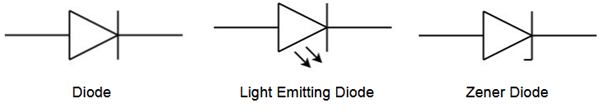
\includegraphics[width=0.7\textwidth]{diode/figurer/oppgave1.png}
	\caption{Eksempel på forskjellige diode symboler.}
	\label{fig:zenBasic}
	\end{figure}

\end{question}


\vspace{0.5cm} % Add space after the solution

\begin{solution}[name=Løsningsforslag oppgave]
A er andode mens B er katode.

\end{solution}

\begin{question}[name=Oppgave, topic=zenerdioder]
En zenerdiode er merket 6V2/3W. Hva er den maksimale strømmen zenerdioden kan tåle?
\end{question}

\vspace{0.5cm} % Add space after the solution

\begin{solution}[name=Løsningsforslag oppgave]
\[P=U\cdot I\rightarrow I=\frac{P}{U}=\frac{3}{6,2}=484 [mA]\]
	
\end{solution}



\begin{question}[name=Oppgave, topic=zenerdioder]
En likespenning som varierer mellom $18 [V]$ og $24 [V]$ skal benyttes for å generere en stabil likespenning på $7,5 [V]$. Kretsen skal benytte en zenerdiode som tåler en effekt på $4 [W]$.

\begin{enumerate}[label=\roman*]
	\item Tegn opp kretsen
	\item Beregn den minste verdien seriemotstanden kan ha
	\item Beregn størrelsen på strømmen det maksimalt kan trekkes fra den stabiliserte spenningen på utgangen, før utgangsspenningen avviker fra $7,5 [A]$
\end{enumerate}
\end{question}

\vspace{0.5cm} % Add space after the solution

\begin{solution}[name=Løsningsforslag oppgave]
\begin{enumerate}[label=\roman*]
	\item Figur \ref{fig:zenKrets1} viser ett eksempel på hvordan kretsen kan tegnes.
		\begin{figure}[H]
			\centering
			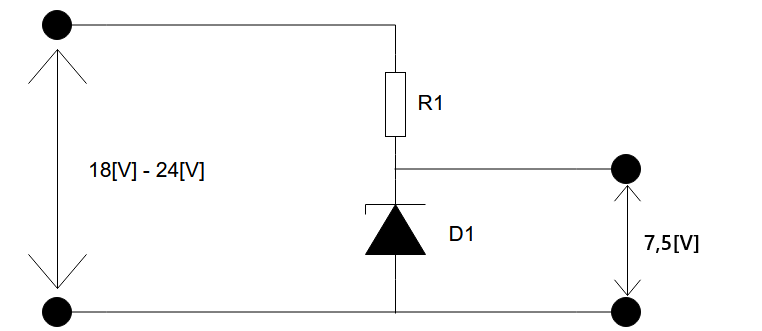
\includegraphics[width=0.7\textwidth]{diode/figurer/zenKrets1.png}
			\caption{Eksempel på forskjellige diode symboler.}
			\label{fig:zenKrets1}
		\end{figure}
	\item Beregner den minste verdien motstanden kan ha slik at strømmen i kretsen ikke blir større enn hva zenerdioden tåler.
	\[I_{D_{maks}}=\frac{P}{U_{maks}}=\frac{4}{7,5}=\frac{8}{15}\approx 0,53 [V]\]
	\item 

\end{enumerate}

	
\end{solution}


\begin{question}[name=Oppgave, topic=zenerdioder]
	
\end{question}

\vspace{0.5cm} % Add space after the solution

\begin{solution}[name=Løsningsforslag oppgave]
	
	
\end{solution}


\begin{question}[name=Oppgave, topic=zenerdioder]
	
\end{question}

\vspace{0.5cm} % Add space after the solution

\begin{solution}[name=Løsningsforslag oppgave]
	
	
\end{solution}



\begin{question}[name=Oppgave, topic=zenerdioder]
	
\end{question}

\vspace{0.5cm} % Add space after the solution

\begin{solution}[name=Løsningsforslag oppgave]
	
	
\end{solution}



\begin{question}[name=Oppgave, topic=zenerdioder]
	
\end{question}

\vspace{0.5cm} % Add space after the solution

\begin{solution}[name=Løsningsforslag oppgave]
	
	
\end{solution}



\begin{question}[name=Oppgave, topic=zenerdioder]
	
\end{question}

\vspace{0.5cm} % Add space after the solution

\begin{solution}[name=Løsningsforslag oppgave]
	
	
\end{solution}



\begin{question}[name=Oppgave, topic=zenerdioder]
	
\end{question}

\vspace{0.5cm} % Add space after the solution

\begin{solution}[name=Løsningsforslag oppgave]
	
	
\end{solution}



\begin{question}[name=Oppgave, topic=zenerdioder]
	
\end{question}

\vspace{0.5cm} % Add space after the solution

\begin{solution}[name=Løsningsforslag oppgave]
	
	
\end{solution}



\begin{question}[name=Oppgave, topic=zenerdioder]
	
\end{question}

\vspace{0.5cm} % Add space after the solution

\begin{solution}[name=Løsningsforslag oppgave]
	
	
\end{solution}



\begin{question}[name=Oppgave, topic=zenerdioder]
	
\end{question}

\vspace{0.5cm} % Add space after the solution

\begin{solution}[name=Løsningsforslag oppgave]
	
	
\end{solution}



\begin{question}[name=Oppgave, topic=zenerdioder]
	
\end{question}

\vspace{0.5cm} % Add space after the solution

\begin{solution}[name=Løsningsforslag oppgave]
	
	
\end{solution}



\begin{question}[name=Oppgave, topic=zenerdioder]
	
\end{question}

\vspace{0.5cm} % Add space after the solution

\begin{solution}[name=Løsningsforslag oppgave]
	
	
\end{solution}


